
\section{Resultate}\label{Chap_results}

Wie angekündigt möchten wir in diesem abschließenden Abschnitt die Resultate aus unserer Programmierung analysieren. Wir haben mehrere Problemgitter und Kombinationen aus Verfahren getestet, und dabei die Daten aufbereitet. Diese Daten werden samt dem Programm bei der Abgabe zur Verfügung gestellt.
Wir haben uns für die Analyse der Verfahren für zwei Testprobleme entschieden. Zum einen soll ein kleiner Kreis zu einem großen Kreis deformiert werden, wobei die Kreismittelpunkte jeweils gleich bleiben. Somit handelt es sich bei diesem Problem um eine Deformation einer konvexen Form ohne große Translation. Zum anderen soll ein kleiner Kreis zu einer nierenartigen Form deformiert werden. In diesem Problem findet eine verhältnismäßig starke Translation statt, außerdem ist die Zielform ein nicht konvex, was dieses Problem deutlich schwieriger als das erste macht. In beiden Fällen sind die Formen in dem Einheitsquadrat im $\mathbb{R}^2$ eingebettet. Diese sind zu sehen in Abbildung \ref{Meshes}. 
Die Parameter, welche bei der Analyse in Betracht kommen, sind als Standard auf folgende Werte gesetzt:
\begin{align*}
\text{Gitterfeinheit: \hspace{0.2cm} }& 0.1 \text{ (normal)} \hspace{0.65cm} ,0.025 \text{ (fein)} \\
\text{Lamé-Parameter: \hspace{0.2cm} }& 0.0 \text{ (min)} \hspace{1.2cm}  ,30.0 \text{ (max)} \\
\text{Perimeter-Reg.: \hspace{0.2cm} }& 0.00001 \\
\text{Funktionswerte für Zustand: \hspace{0.2cm} }& -10.0 \text{ (außen) },  100.0 \text{ (innen)} \\
\text{Memory-Length: \hspace{0.2cm} }& 60 \\
\text{Toleranz für Ausstieg: \hspace{0.2cm} }& 0.0008 \\
\text{Backtracking: \hspace{0.2cm} }& 5.0 \text{ (start\_scale)}, 0.5 \text{ (shrinkage)}, 0.999 \text{ (c)}
\end{align*}

\begin{figure}
	\begin{subfigure}{0.5\textwidth}
	\centering
	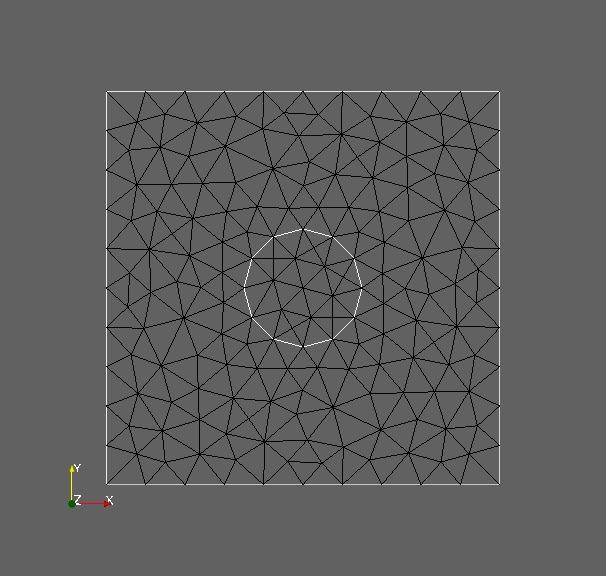
\includegraphics[scale=0.25]{pic_smallcircle.jpg}
	\caption{}	
	\end{subfigure}
	\begin{subfigure}{0.5\textwidth}
	\centering
	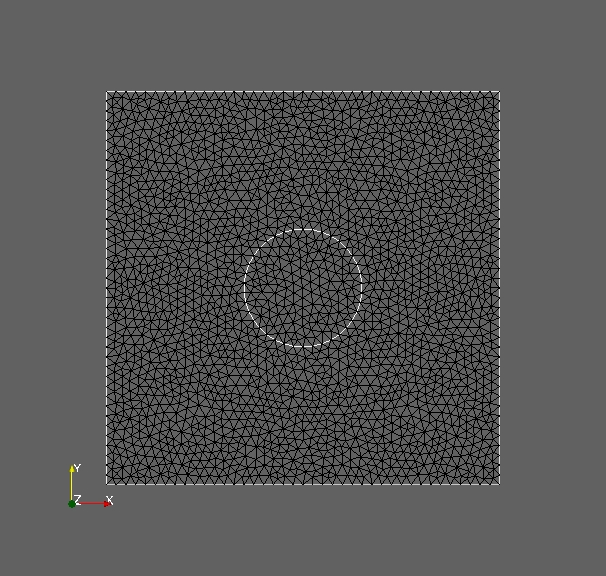
\includegraphics[scale=0.25]{pic_smallcircle_fine.jpg}
	\caption{}	
	\end{subfigure}
	\begin{subfigure}{0.5\textwidth}
	\centering
	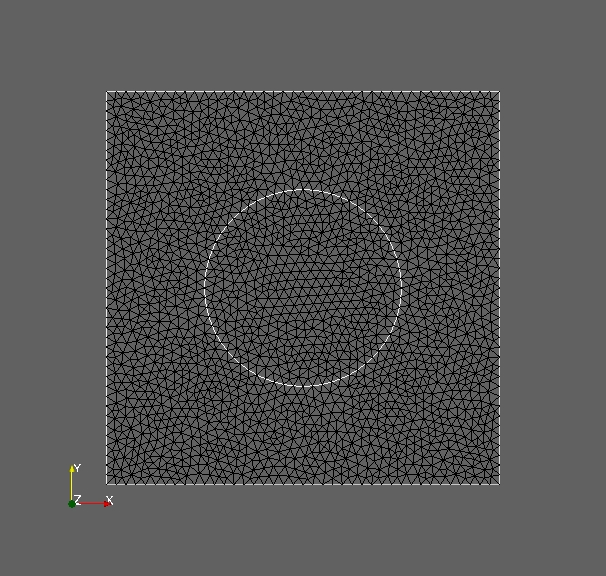
\includegraphics[scale=0.25]{pic_bigcircle_fine.jpg}
	\caption{}	
	\end{subfigure}
	\begin{subfigure}{0.5\textwidth}
	\centering
	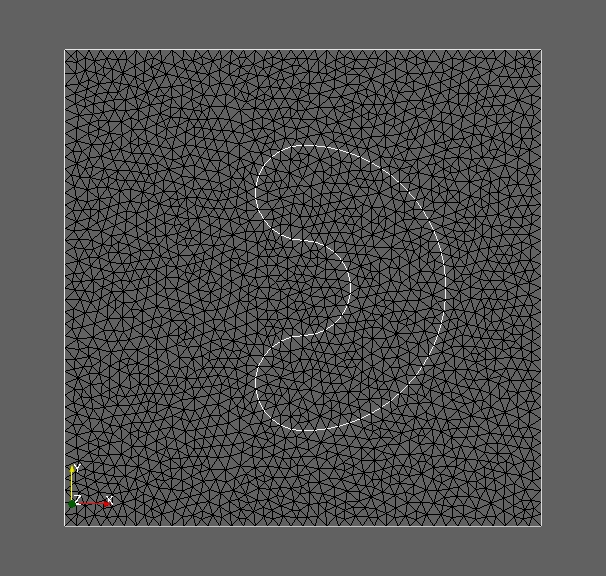
\includegraphics[scale=0.25]{pic_brokendonut_fine.jpg}
	\caption{}	
	\end{subfigure}
\caption{(a) Ausgangsform kleiner Kreis auf grobem Gitter (b) Ausgangsform kleiner Kreis auf feinem Gitter (c) Zielform großer Kreis auf feinem Gitter (d) Zielform Broken Donut auf feinem Gitter}
\label{Meshes}
\end{figure}

Wir werden sowohl das L-BFGS-Verfahren, als auch das Gradientenverfahren vergleichen. Außerdem wird jeweils die Linesearch an- und ausgeschaltet, sowie alle oben aufgeführten Parameter, bis auf die Funktionswerte die Zustandsgleichung im Zielgitter, den Verbesserungsfaktor \textsf{c}, und den Skalierungsfaktor \textsf{shrinkage} der Backtracking-Linesearch, variiert. Die Verwendung der Memory-Length von 60 bewirkt, dass es sich in allen folgenden Fällen der Verwendung des L-BFGS-Verfahrens eigentlich um ein BFGS-Verfahren handelt, da die gesamte Historie zur Berechnung der Hesse-Approximation benutzt wird. 

\subsection{Problem: kleiner zu großem Kreis}\label{subsect_circle}

Für das Problem der Deformation zum großen Kreis betrachten wir vor dem BFGS-Verfahren zunächst das Gradientenverfahren. Alle Zeiten und Anzahlen der benötigten Schritte der Verfahren finden sind in Tabelle \ref{Tabelle}. Wir erhalten bei dem groben Gitter 
bei Verwendung des Gradientenverfahrens ohne Linesearch Konvergenz nach fast 800 Schritten. Schaltet man das Backtracking ein, so erhält man ebenfalls Konvergenz, jedoch bei gut halber Anzahl der Schritte. Dies legt nahe, das die Schrittweite durch das anfängliche Hochskalieren der Deformation optimaler wird, der Gradient also der Norm nach relativ klein war. Bei Verfeinerung des Gitters um das 4-fache erhalten wir ebenfalls ohne Verwendung der Linesearch beim Gradientenverfahren Konvergenz nach ca. 650 Schritten, wobei wieder durch Verwendung des Backtracking eine Beschleunigung zur Konvergenz stattfindet. Die Konvergenzplots finden sich in Abbildung \ref{Konvplots_circle}. Erhöht man das anfängliche Hochskalieren vom Faktor 5 auf 20, so erhält man im feinen Gitter Konvergenz schon nach 120 Schritten. Die Geschwindigkeit zur Konvergenz hat sich also im Vergleich zum Gradientenverfahren ohne Backtracking also um das 5-fache gesteigert, wobei sich die erzeugten Gitter bei Ausstieg des Verfahrens mit oder ohne Linesearch und Veränderung des Hochskalierungsfaktors so gut wie nicht unterscheiden. 

\begin{table}[h]
\centering
\begin{tabular}{c rrrr}
\hline\\[-2.5ex]
 & \hspace{1cm} Zeit & & \hspace{1cm} Schritte \\
Problem &Gradientenv. &BFGS-Verf. &Gradientenv. &BFGS-Verf.  \\[0.2ex]

\hline \hline 
großer Kreis (grob) & 13,7s      & 4,8s       & 33      & 6 \\
großer Kreis (fein) & 1min 31,3s & 17,2s      & 52      & 7 \\
Broken Donut (grob) & 43,3s$^*$  & 6,6s       & 109$^*$ & 9 \\
Broken Donut (fein) & 27min 4,6s & 1min 25,4s & 910     & 27 \\
\hline
\end{tabular} 

\vspace{0.2cm}$^*$ \textit{Gradientenverfahren steigt bei Genauigkeit 0.0033 aus, weil \newline \hspace{-3.2cm}Linesearch keine Abstiegsrichtung findet}
 
\caption{Rechendauern und Schritte der Verfahren (mit Backtracking-Linesearch)}
\label{Tabelle}

\end{table}

Findet das BFGS-Verfahren ohne Linesearch Anwendung, so erhält man auf dem groben Gitter keine Konvergenz. Das Verfahren updatet die BFGS-Memory nach mehreren Verletzungen der Curvature Condition nicht, und deformiert das Gebiet schließlich bei Schritt 26 bis zur Unbrauchbarkeit, was in Abbildung \ref{Destroyedbfgs_grob} zu sehen ist. Man beachte die starke Entartung der kaum sichtbaren Zellen kurz vor der Zerstörung des Gitters, welche man im Zoom gut erkennt.


\begin{figure}
	\begin{subfigure}{0.5\textwidth}
	\centering
	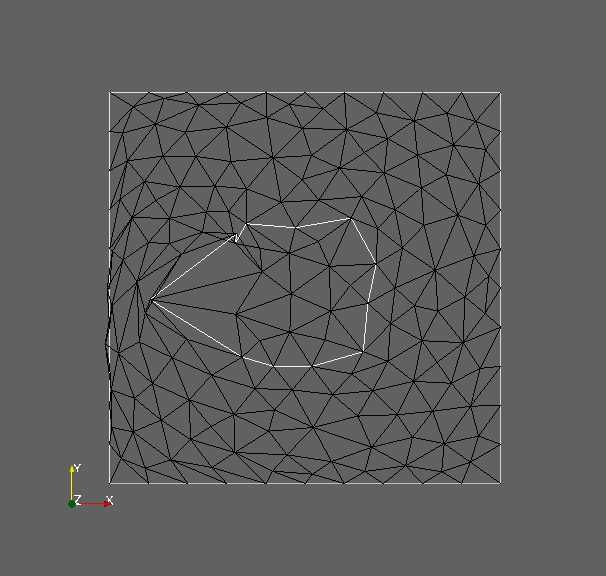
\includegraphics[scale=0.25]{pic_smallcircle_destroyed1.jpg}
	\caption{}	
	\end{subfigure}
	\begin{subfigure}{0.5\textwidth}
	\centering
	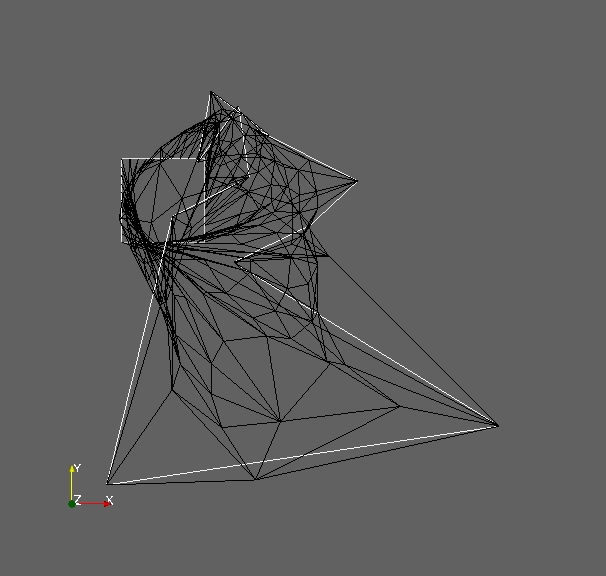
\includegraphics[scale=0.25]{pic_smallcircle_destroyed2.jpg}
	\caption{}	
	\end{subfigure}
\caption{(a) Gitter nach mehrmaligen Schritten unter Verletzung der Curvature Condition und Non-Update Schritten (b) der darauf folgende Schritt, Zerstörung des Gitters}
\label{Destroyedbfgs_grob}
\end{figure}

Auch bei Verfeinerung des Gitters um das 4-fache erhält man keine Konvergenz des BFGS-Verfahrens, sondern erreicht die Zerstörung des Gitters nach Verletzung der Curvature Condition schon im zweiten Schritt, bei der die Form das Einheitsquadrat verlässt, siehe Abbildung \ref{Destroyedbfgs}. Man beachte, das dieses mal die Richtung des Schrittes in Richtung Optimum geht, jedoch viel zu lang ist, anders als in Abbildung \ref{Destroyedbfgs_grob}, wo zuvor mehrmalige falsche Schritte bei Verletzung der Curvature Condition das grobe Gitter zerstören. Diese Beobachtung macht erneut deutlich, wie wichtig eine effektive Schrittweitensteuerung bei der Implementierung der Verfahren ist.

\begin{figure}
	\begin{subfigure}{0.5\textwidth}
	\centering
	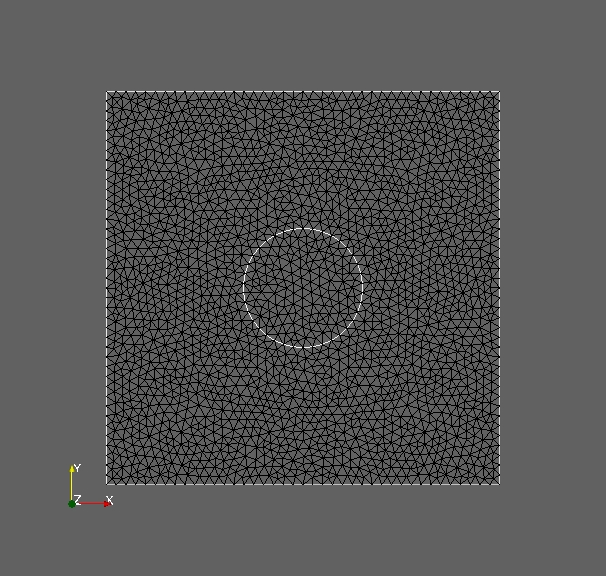
\includegraphics[scale=0.25]{pic_smallcircle_bfgsdestroyed1.jpg}
	\caption{}	
	\end{subfigure}
	\begin{subfigure}{0.5\textwidth}
	\centering
	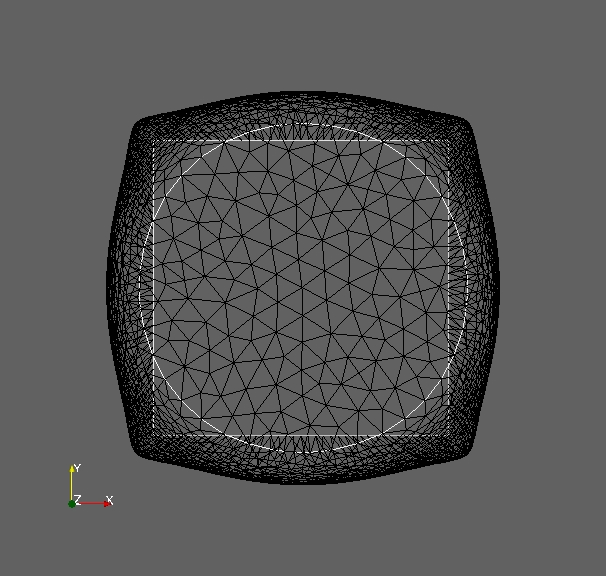
\includegraphics[scale=0.25]{pic_smallcircle_bfgsdestroyed2.jpg}
	\caption{}	
	\end{subfigure}
\caption{(a) 1. Schritt des BFGS-Verfahrens: Gradientenschritt bei feinem Gitter (b) 2. Schritt: BFGS-Schritt mit Entartung des feinen Gitters}
\label{Destroyedbfgs}
\end{figure}

Wir haben auch versucht, die Gitterzerstörung beim BFGS-Verfahren durch Modifikation der lokal variierenden Lamé-Parameter zu begegnen. Alle bisher gezeigten Gitter hatten die Wahl des minimalen Lamé-Parameters von 0. Um zu beobachten, ob die Verfahren instabiler werden, wenn man konstante Lamé-Parameter wählt, haben wir diese konstant auf 30 gesetzt. Man erhält den Output \ref{Destroyedkonstlame}, wobei bei Schritt 5 und 6 die Curvature Condition verletzt sind, und keine Linesearch verwendet wurde.

\begin{figure}
	\begin{subfigure}{0.3\textwidth}
	\centering
	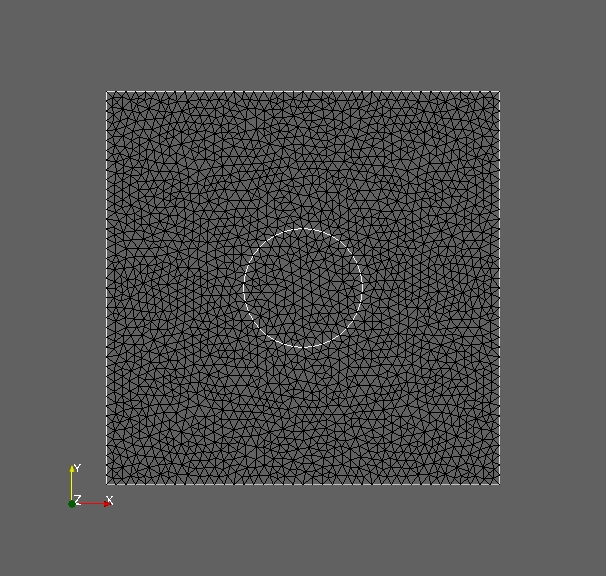
\includegraphics[scale=0.2]{pic_bigcircle_constlame1.jpg}
	\caption{}	
	\centering
	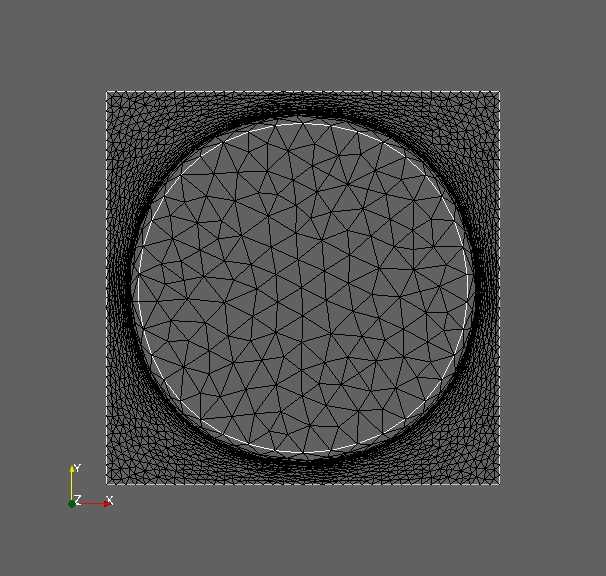
\includegraphics[scale=0.2]{pic_bigcircle_constlame2.jpg}
	\caption{}	
	\end{subfigure}
	\begin{subfigure}{0.3\textwidth}
	\centering
	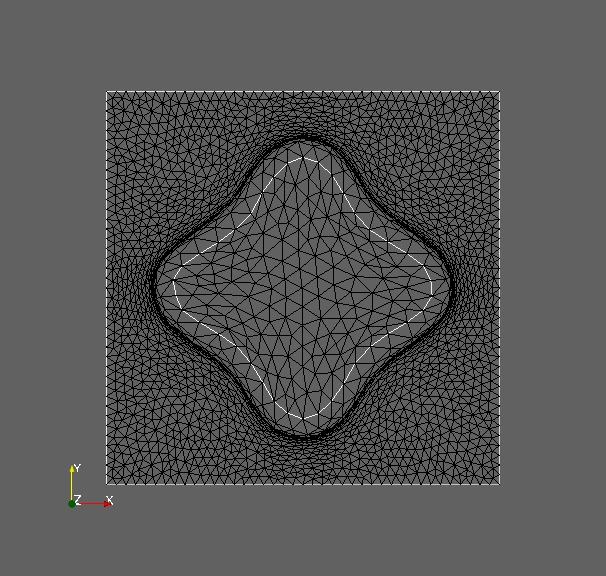
\includegraphics[scale=0.2]{pic_bigcircle_constlame3.jpg}
	\caption{}	
	\centering
	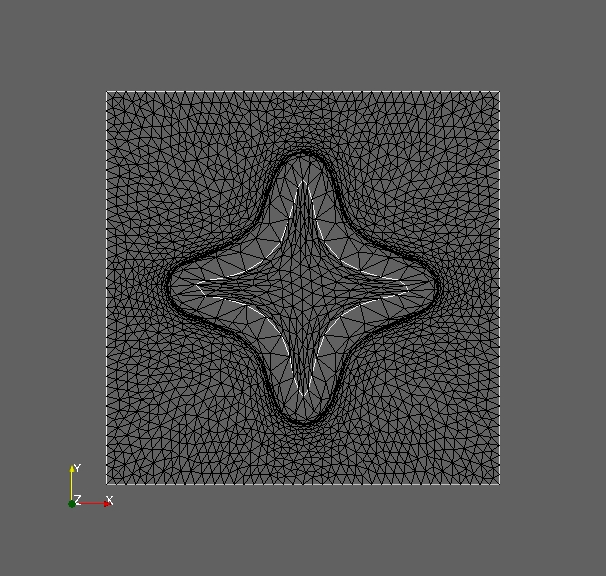
\includegraphics[scale=0.2]{pic_bigcircle_constlame4.jpg}
	\caption{}	
	\end{subfigure}
	\begin{subfigure}{0.3\textwidth}
	\centering
	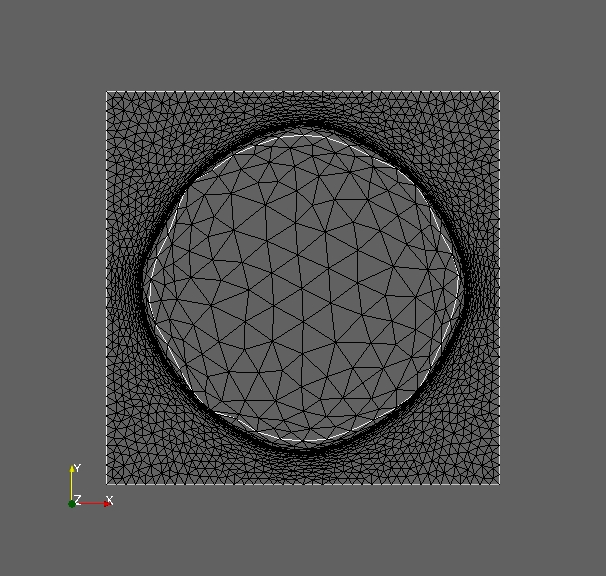
\includegraphics[scale=0.2]{pic_bigcircle_constlame5.jpg}
	\caption{}	
	\centering
	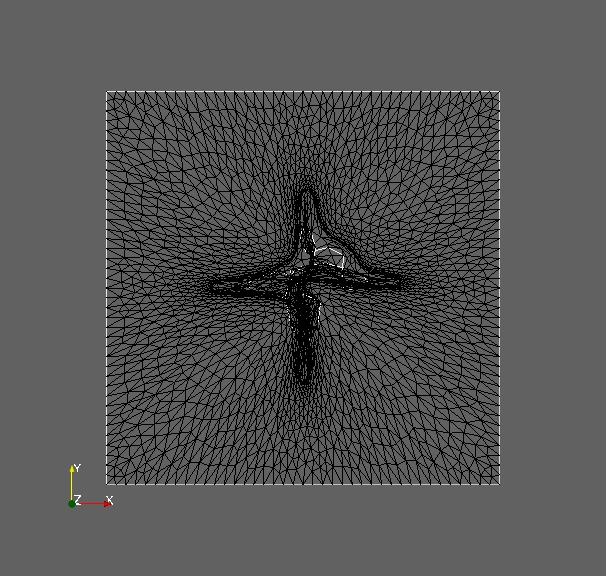
\includegraphics[scale=0.2]{pic_bigcircle_constlame6.jpg}
	\caption{}	
	\end{subfigure}
\caption{BFGS-Verfahren ohne Schrittweitensteuerung bei konstanten Lamé-Parametern mit Wert 30; die ersten 6 Schritte}
\label{Destroyedkonstlame}
\end{figure}

Ein komplett anderes Verhalten stellt sich bei Verwendung der Backtracking-Linesearch ein; in diesem Fall konvergiert das L-BFGS-Verfahren für beide Gitterfeinheiten.
Zudem fällt eine erhebliche Steigerung der Konvergenzgeschwindigkeit im Vergleich zum Gradientenverfahren auf; schon nach 5 Schritten auf dem groben, und nach 6 auf dem feinen Gitter. Die entsprechenden Konvergenzplots für die Verfahren mit Linesearch auf grobem und feinem Gitter sind zu sehen in \ref{Konvplots_circle}.

\begin{figure}
	\begin{subfigure}{0.5\textwidth}
	\centering
	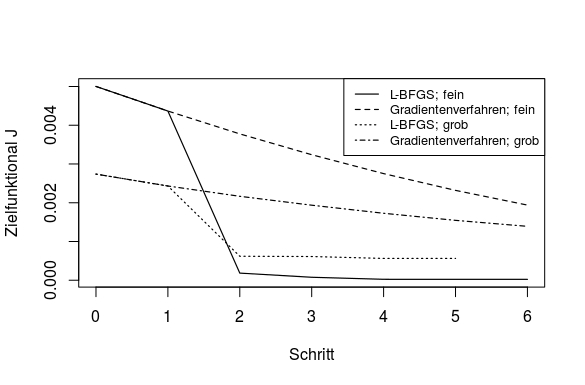
\includegraphics[scale=0.48]{plot_circle_target.jpeg}
	\caption{}	
	\end{subfigure}
	\begin{subfigure}{0.5\textwidth}
	\centering
	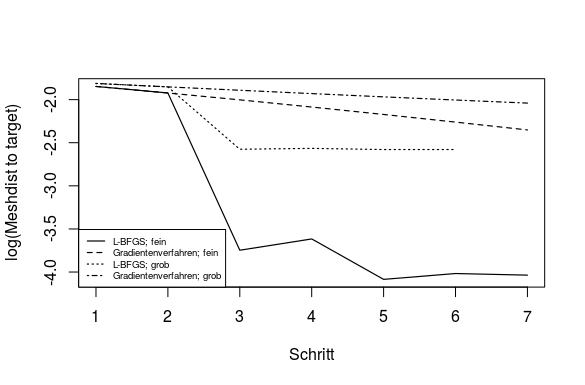
\includegraphics[scale=0.48]{plot_circle_meshdist.jpeg}
	\caption{}	
	\end{subfigure}
\caption{kleiner Kreis auf großer Kreis (a) Werte des Zielfunktionals bei den Verfahren mit Linesearch; unterschiedliche Gitterfeinheiten (b) logarithmierte Meshdistanz bei Verfahren mit Linesearch; unterschiedliche Gitterfeinheiten}
\label{Konvplots_circle}
\end{figure}

Die bei dem groben Gitter erzeugte optimale Form besitzt noch einen mit bloßem Auge sichtbaren Abstand zur Zielform. In diesem Fall hat unser L-BFGS-Algorithmus bei dem Backtracking maximal herunterskaliert, d.h. keine Abstiegsrichtung gefunden und ist ausgestiegen. Damit scheint ein lokales Minimum erreicht, zu sehen in Abbildung  \ref{Konvergenzbfgscircle} (a). Diese Vermutung liegt nahe, da die zugehörigen Werte der Norm der Formableitung \textsf{nrm\_f\_elas} gegen Null streben, hierzu verweisen wir auf die mitgelieferten Daten. Bei Verwendung des feinen Gitters ist bei selbem Ausstiegskriterium kein Abstand zur Zielform sichtbar, was man in Abbildung \ref{Konvergenzbfgscircle} (b) sehen kann.

\begin{figure}
	\begin{subfigure}{0.5\textwidth}
	\centering
	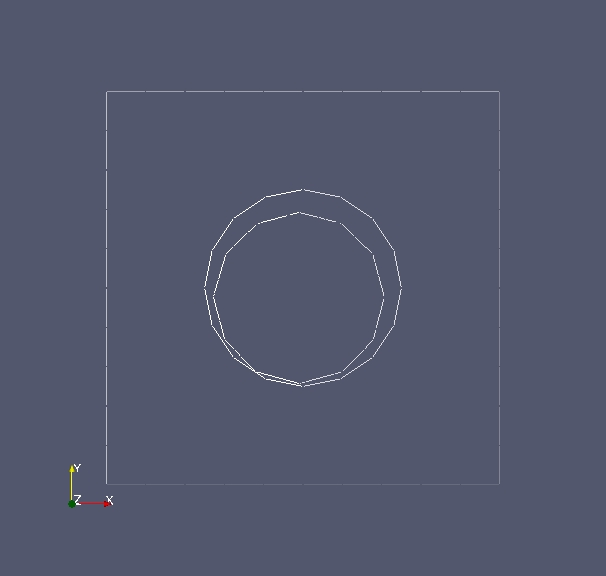
\includegraphics[scale=0.25]{pic_bigcircle_bfgs_linesearch.jpg}
	\caption{}	
	\end{subfigure}
	\begin{subfigure}{0.5\textwidth}
	\centering
	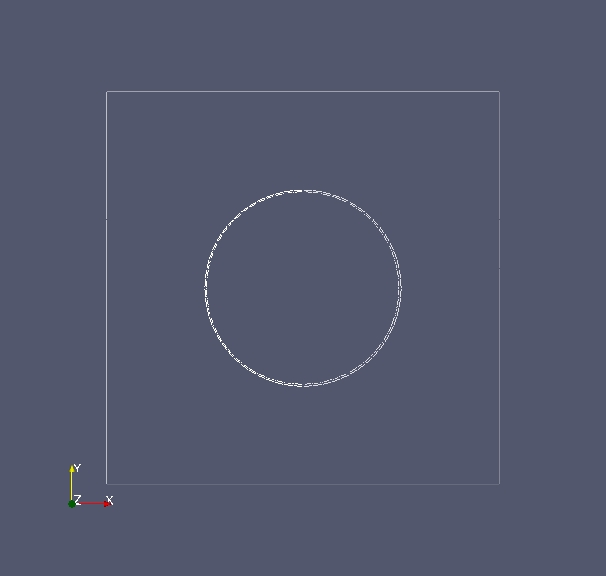
\includegraphics[scale=0.25]{pic_bigcircle_bfgs_linesearch_fine.jpg}
	\caption{}	
	\end{subfigure}
\caption{(a) L-BFGS mit Backtracking bei grobem Gitter. Abweichung bei Ausstieg sichtbar. (b) L-BFGS mit Backtracking bei feinem Gitter. Abweichung bei Ausstieg nicht erkennbar.}
\label{Konvergenzbfgscircle}
\end{figure}

Wir haben durch Veränderung der Perimeter-Regularisierung untersucht, ob sich durch diese der Abstand zur Zielform erklären lässt. Die Vermutung ist, dass die optimale Form etwas kleiner als die Zielform ist, da die Perimeter-Regularisierung kleinere Formen favorisiert. Die in diesem Fall entstehende optimale Lösung ist in diesem Fall symmetrisch mit gleichem Mittelpunkt wie die Zielform, jedoch besitzt sie fast den selben Abstand wie die optimale Form mit der Perimeter-Regularisierung aus Abbildung \ref{Konvergenzbfgscircle} (a). Für die exakten Bilder verweisen wir auf die mitgelieferten \textsf{.pvd}-Dateien.

Kontrollieren wir im Falle des BFGS-Algorithmus auf Veränderung bei Erhöhung des Hochskalierungsfaktors \textsf{starscale} des Backtracking, so stellen wir fest, dass die ersten Schritte stärkere Verbesserungen bringen. Sobald sich jedoch eine gewisse Memorygröße, und damit eine Hesse-Approximation, aufgebaut haben, verschwinden diese Effekte wieder, siehe Abbildung \ref{plot_startscales}. Dieses Verhalten sollte auftreten, da BFGS-Schritte mit aufgebauter Hesse-Approximation skalierungsinvariant sind.

\begin{figure}
	\begin{subfigure}{0.5\textwidth}
	\centering
	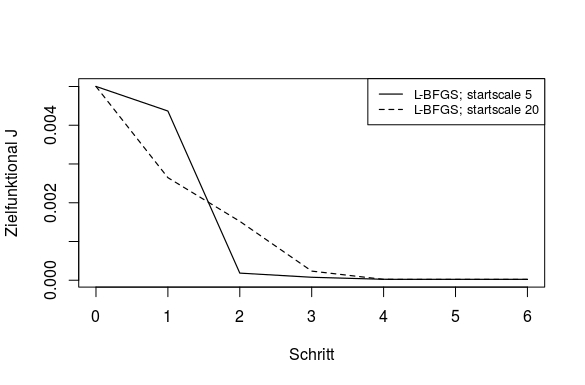
\includegraphics[scale=0.48]{plot_circle_bfgs_fine_startscale.jpeg}
	\caption{}	
	\end{subfigure}
	\begin{subfigure}{0.5\textwidth}
	\centering
	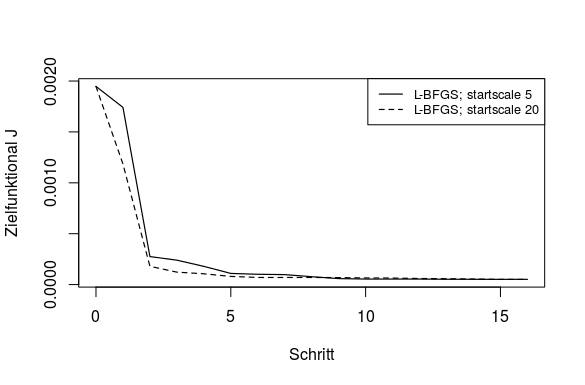
\includegraphics[scale=0.48]{plot_donut_bfgs_fine_startscale.jpeg}
	\caption{}	
	\end{subfigure}
\caption{Zielfunktional bei Variation des Skalierungsparameters \textsf{start\_scale} des Backtracking für das L-BFGS-Verfahren auf feinen Gittern der Probleme
 (a) kleiner Kreis auf großen Kreis (b) kleiner Kreis auf "Broken  Donut"}
\label{plot_startscales}
\end{figure}

Zudem haben wir einen Vergleich zwischen der vollen BFGS-Methode, welche wir durch die \textsf{memory\_length} von 60 erzeugen, und der echten Limited-Memory-BFGS-Methode, mit \textsf{memory\_length} von 2 und 3, im Falle des feinen Gitters gezogen. Interessanterweise stellt sich hier überhaupt kein Unterschied hinsichtlich Konvergenzgeschwindigkeit und erzeugte Werte im Zielfunktional ein, was man in Abbildung \ref{plot_memlen_lame} (a) erkennen kann. Ähnliche Beobachtungen machten die Autoren von \cite{diffusion} bei elliptischen und parabolischen Problemen, siehe das genannte Paper, Abschnitt 3. Dies lässt sich nach unserer Vermutung dadurch erklären, dass für einen korrekten BFGS-Schritt ein Term fehlt. Würde dieser ergänzt, so hoffen wir auf eine Verbesserung des Algorithmus bei höherer \textsf{memory\_length} auftreten sollte. Außerdem lässt sich in den Diagrammen keine asymptotische superlineare Konvergenz nachweisen, welche sich bei korrektem Update möglicherweise einstellt.

\begin{figure}
	\begin{subfigure}{0.5\textwidth}
	\centering
	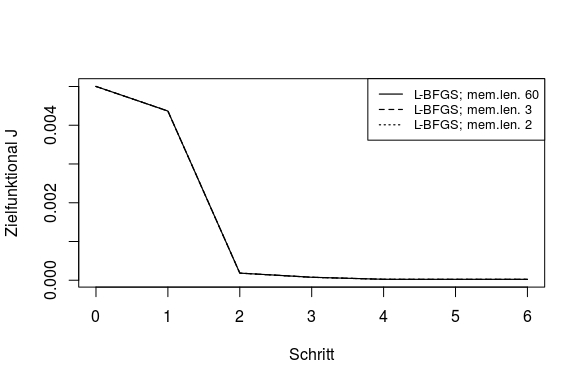
\includegraphics[scale=0.48]{plot_circle_bfgs_fine_memlen.jpeg}
	\caption{}	
	\end{subfigure}
	\begin{subfigure}{0.5\textwidth}
	\centering
	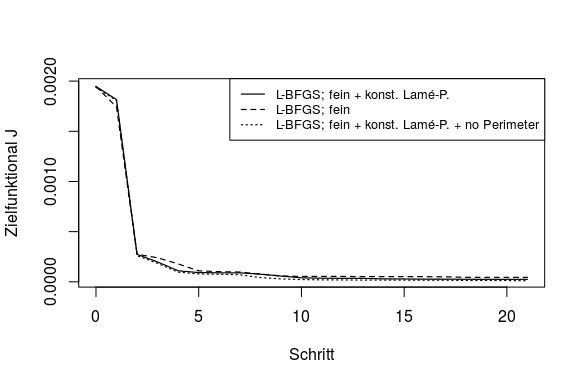
\includegraphics[scale=0.48]{plot_donut_bfgs_fine_lame.jpeg}
	\caption{}	
	\end{subfigure}
\caption{(a) Variation des L-BFGS-Parameters \textsf{memory\_length} bei feinem Gitter des Problems kleiner Kreis auf großer Kreis. Zu sehen sind 3 verschiedene Graphen, numerische Abweichungen treten erst ab Schritt 5 ab der 3 Nachkommastelle auf, weshalb diese fast gleich aussehen. \newline (b) Änderung der Lamé-Parameter und Entfernen der Perimeter-Regularisierung auf feinem Gitter des Problems kleiner Kreis auf "Broken  Donut".}
\label{plot_memlen_lame}
\end{figure}

Neben der bloßen Bedingung einer Verbesserung im Zielfunktional bei dem Backtracking besteht die Möglichkeit, die Armijo-Bedingung für die Linesearch zu verwenden. Diese haben wir nach \cite{Nocedal}, wie im Unterabschnitt  \ref{backtracking} gezeigt,  implementiert. Verwendet man diese, so konvergiert die L-BFGS-Methode nicht mehr, in einigen Fällen konvergiert das Gradientenverfahren. Jedoch würde wir eher behaupten, dass dies \textit{trotz} der Armijo-Bedingung konvergiert. Da diese Bedingung die Verbesserung mit Hilfe eines linearen Modells in der aktuellen Form betrachtet, wäre ein aus der Formoptimierung legitimes anderes Modell vorstellbar, um verbesserte Bedingungen zur Linesearch zu erzeugen. Hierzu hat uns leider die Zeit gefehlt.

Bei der Berechnung des Formgradienten, wie im Unterabschnitt \ref{Berechnung_bib} erklärt, haben wir ein Verfahren verwendet, welches in der linearen Elastizitätsgleichung die Punkte, welche nicht Träger des inneren Randes sind, auf Null setzt. Schaltet man diese Nullsetzung aus, was durch die Wahl des Parameters \textsf{zeroed = False} möglich ist, so zerstört dies die Konvergenz des Verfahrens. Sowohl das L-BFGS, als auch das Gradientenverfahren divergieren in allen von uns getesteten Beispielen. Somit tritt der selbe Effekt wie in \cite{bfgs2}, welcher dort in Abschnitt 5, Fig. 2 zu sehen ist. Würde dieser Effekt durch ein Rundungsrauschen hervorgerufen sein, so vermuten wir, dass dieses weniger drastisch sichtbar würde. Bei uns ist schon nach den ersten Schritten das Gitter bis zur Unbrauchbarkeit entartet. Eine befriedigende Erklärung hierfür haben wir leider nicht.

\subsection{Problem: kleiner Kreis zu 'Broken Donut'}\label{subsect_donut}

Wir haben die oben genannten Beobachtungen auch für das schwierigere Problem der nierenförmigen, nicht konvexen Form gesammelt. Die Ausgangsform, welcher den kleinen Kreis in Abbildung \ref{Meshes} (a) und (b) darstellt, bleibt gleich, wir wechseln also nur die Zielform, die auch in Abbildung \ref{Meshes} (d) zu sehen ist. 

Anders als bei dem einfacheren ersten Problem, erhalten wir für ein Gradientenverfahren ohne Backtracking-Linesearch, in den Fällen sowohl des groben, als auch des feinen Gitters, nach ca. 1200, respektive ca. 600 Schritten zwar Konvergenz, jedoch nicht zum globalen Optimum des Zielgitters. Wir vermuten, dass es sich hierbei um lokale Minima handelt, weil die Norm der Formableitung \textsf{nrm\_f\_elas} gegen $0$ geht, wobei wir auf die Daten verweisen. Die resultierende optimale Form bleibt konvex, trotz des nicht konvexen Zielgitters, siehe Abbildung
\ref{brokendonutgradient}. 

\begin{figure}
	\begin{subfigure}{0.5\textwidth}
	\centering
	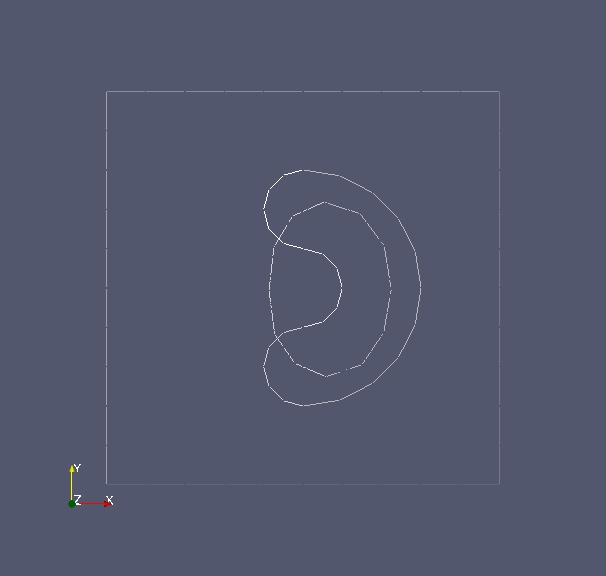
\includegraphics[scale=0.25]{pic_brokendonut_gradient.jpg}
	\caption{}	
	\end{subfigure}
	\begin{subfigure}{0.5\textwidth}
	\centering
	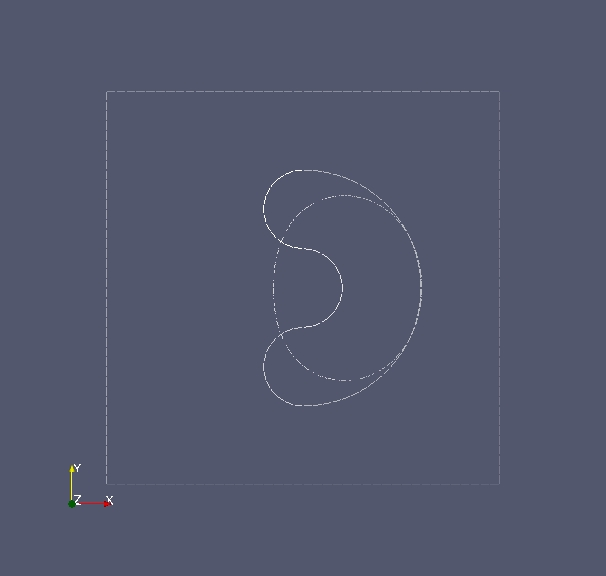
\includegraphics[scale=0.25]{pic_brokendonut_gradient_fine.jpg}
	\caption{}	
	\end{subfigure}
\caption{(a) Optimale Form und Zielform bei Gradientenverfahren auf grobem Gitter (b) Selbiges auf feinem Gitter}
\label{brokendonutgradient}
\end{figure}

Durch das Verwenden der Backtracking-Linesearch schafft es der Algorithmus näher an das globale Optimum zu gelangen. Dies gelingt jedoch ausschließlich bei dem feinen Gitter. Im Falle des groben Gitters erreichen wir auch mit Linesearch die selbe nicht konvexe Form, siehe Abbildung \ref{brokendonutgradient_linesearch}, wobei eine leichte Verbesserung zu sehen ist. Dies zeigt, dass das Verfahren abhängig von der Gitterfeinheit ist, wobei Verfeinerungen Verbesserungen liefern. Für die Zeiten und Schritte verweisen wir auf Tabelle \ref{Tabelle}.

Außerdem beobachten wir für das Gradientenverfahren, wie im ersten Problem, ein Skalieren der Konvergenzgeschwindigkeit durch das Hochskalieren der Suchrichtung bei der Backtracking-Linesearch. Wir sparen uns an dieser Stelle die Angabe eines Plots, da dieses Phänomen bekannt ist.
Zudem haben wir in diesem Problem die gleichen Feststellungen bei Verwendung der Armijo-Bedingung bei der Linesearch gemacht, wie bei dem ersten Problem zuvor.

\begin{figure}
	\begin{subfigure}{0.5\textwidth}
	\centering
	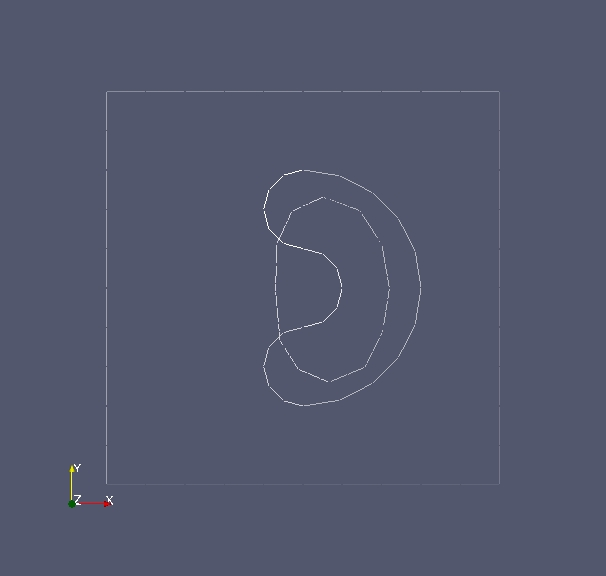
\includegraphics[scale=0.25]{pic_brokendonut_gradient_linesearch.jpg}
	\caption{}	
	\end{subfigure}
	\begin{subfigure}{0.5\textwidth}
	\centering
	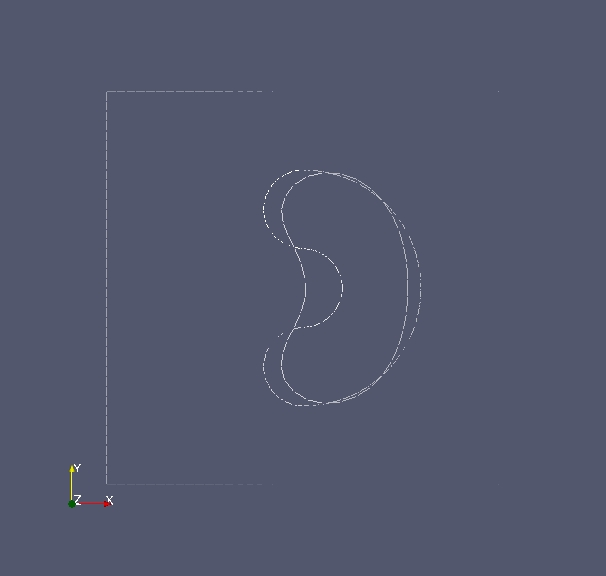
\includegraphics[scale=0.25]{pic_brokendonut_gradient_linesearch_fine.jpg}
	\caption{}	
	\end{subfigure}
\caption{(a) Optimale Form und Zielform bei Gradientenverfahren mit Linesearch auf grobem Gitter (b) Selbiges auf feinem Gitter}
\label{brokendonutgradient_linesearch}
\end{figure}

Bei Verwendung des L-BFGS-Verfahrens ohne Linesearch bemerken wir, ähnlich wie zu dem ersten Beispiel, dass sowohl beim groben, als auch beim feinen Gitter eine zu Abbildung \ref{Destroyedbfgs} ähnliche Divergenz stattfindet, weshalb wir uns Graphiken hierzu sparen. Das Gitter ist nach nur wenigen Schritten, nachdem die Curvature Condition verletzt wurde, bis zur Unkenntlichkeit verformt, wobei das Verfahren auch nicht die lokalen Minima \ref{brokendonutgradient_linesearch} oder \ref{brokendonutgradient} erreicht. 

\begin{figure}
	\begin{subfigure}{0.5\textwidth}
	\centering
	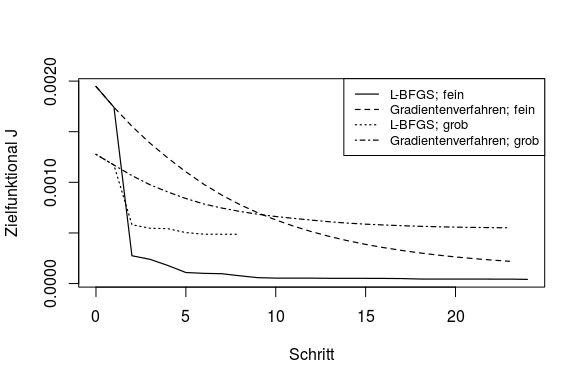
\includegraphics[scale=0.48]{plot_donut_target.jpeg}
	\caption{}	
	\end{subfigure}
	\begin{subfigure}{0.5\textwidth}
	\centering
	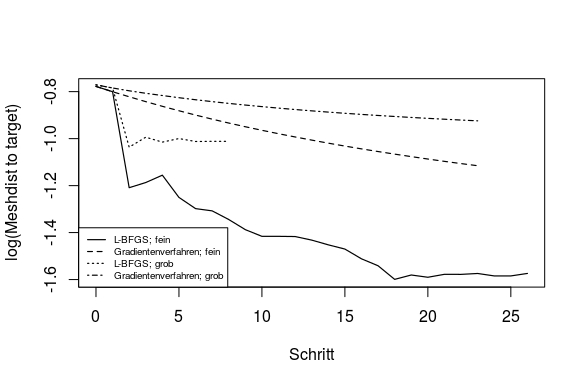
\includegraphics[scale=0.48]{plot_donut_meshdist.jpeg}
	\caption{}	
	\end{subfigure}
\caption{kleiner Kreis auf "Broken Donut" (a) Werte des Zielfunktionals bei den Verfahren mit Linesearch; unterschiedliche Gitterfeinheiten (b) logarithmierte Meshdistanz bei Verfahren mit Linesearch; unterschiedliche Gitterfeinheiten}
\label{plot_konvergenzdonut}
\end{figure}

Interessanterweise verbessert sich das Verhalten des L-BFGS-Verfahrens ohne Linesearch, wenn man statt lokal variierenden Lamé-Parametern konstante Lamé-Parameter mit Wert 30 wählt. Zuvor divergierte das Verfahren bei dem feinen Gitter nach nur 5 Schritten unter Verletzung der Curvature Condition der letzten 3 Schritte. Bei konstanten Lamé-Parametern findet zwar auch Divergenz statt, jedoch erst nach 14 Schritten, wobei zuvor sogar ein optimales Ergebnis, welches dem Gradientenverfahren mit Linesearch auf dem feinen Gitter nahe kommt, erreicht wird. Zu sehen sind ausgewählte Schritte in Abbildung \ref{brokendonut_bfgs_konstlame}. Man beachte jedoch den Vergleich zu dem Gitter, welches bei dem L-BFGS-Verfahren mit Linesearch und variierenden Lamé-Parametern erzeugt wird, bei dem geringere Entartung der Zellen des Gitters zu beobachten sind. Wir würden an dieser Stelle vorschlagen, ein Kriterium für die Entartung des Gitters, etwa dem Quotienten aus maximalem und minimalem Zellvolumen, zu verwenden, um bei Überschreitung eines festgelegten Entartungsgrades ein neues Gitter mit der aktuellen Form zu initialisieren. Dies ließe sich auch mit lokal variierenden Lamé-Parametern, sowie mit adaptiven Gittermethoden, kombinieren.

\begin{figure}
	\begin{subfigure}{0.315\textwidth}
	\centering
	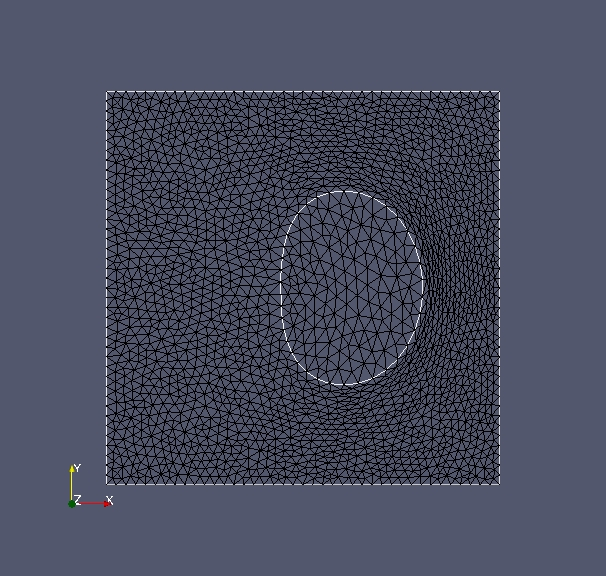
\includegraphics[scale=0.21]{pic_brokendonut_bfgs_konstlame_6.jpg}
	\caption{}	
	\end{subfigure}
	\begin{subfigure}{0.315\textwidth}
	\centering
	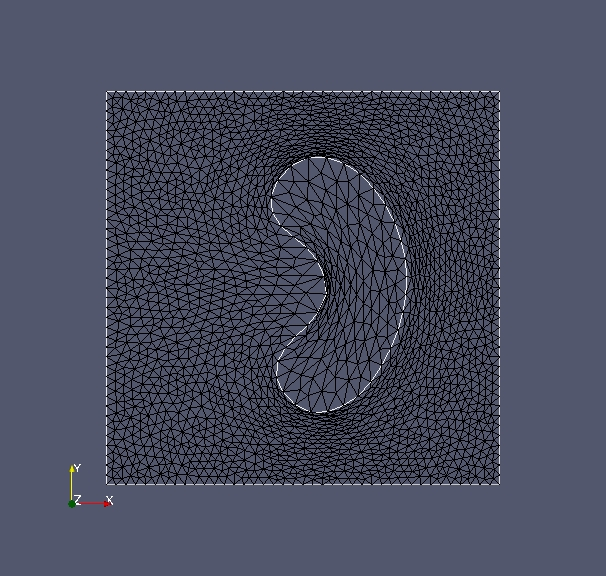
\includegraphics[scale=0.21]{pic_brokendonut_bfgs_konstlame_12.jpg}
	\caption{}	
	\end{subfigure}
	\begin{subfigure}{0.315\textwidth}
	\centering
	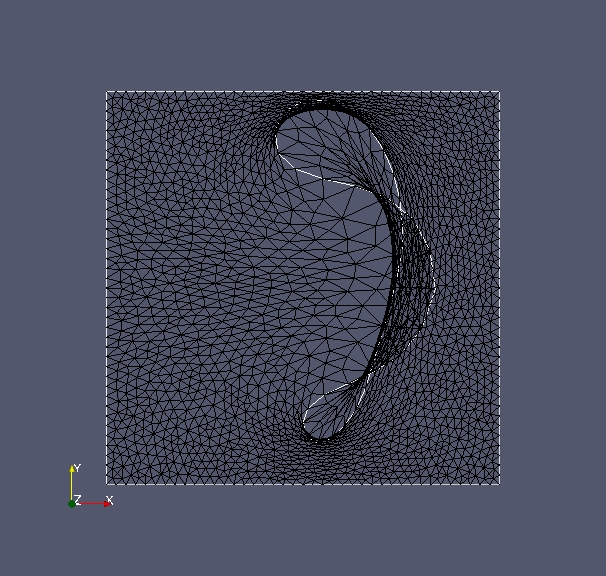
\includegraphics[scale=0.21]{pic_brokendonut_bfgs_konstlame_14.jpg}
	\caption{}	
	\end{subfigure}
\caption{BFGS-Verfahren bei konstanten Lamé-Parameter von 30 (a) Schritt 6 (b) gute Form bei Schritt 12; man beachte die starke Stauchung/ Streckung der Zellen (c) Zerstörung des Gitters bei Schritt 14}
\label{brokendonut_bfgs_konstlame}
\end{figure}

Verwendet man zusammen mit dem L-BFGS-Verfahren die Backtracking-Linesearch, so erhalten wir ähnliche Ergebnisse wie in dem ersten Problem, nämlich eine deutliche Erhöhung der Konvergenzgeschwindigkeit im Vergleich zum Gradientenverfahren auf dem feinen Gitter. Auch auf dem groben Gitter ist eine erhebliche Erhöhung der Konvergenzgeschwindigkeit zu beobachten, wobei auch hier lediglich das lokale Minimum des Gradientenverfahrens erreicht wird. Auf dem feinen Gitter wird, ähnlich dem Gradientenverfahren mit Linesearch, eine sehr gute Lösung erreicht, nahe des globalen Optimums. Zu sehen sind die Ergebnisse des BFGS-Verfahrens mit Linesearch in Abbildung \ref{brokendonut_bfgs_linesearch}, für die Zeiten und Schritte verweisen wir erneut auf Tabelle \ref{Tabelle}. Bei dem Gradientenverfahren ist bei beiden untersuchten Problemen zu erkennen, dass eine deutliche Verfeinerung des Gitters keine Verlangsamung der Konvergenz mit sich bringt, was ein Indiz für gitterunabhängige Konvergenz ist, siehe Abbildung \ref{plot_konvergenzdonut} und \ref{Konvplots_circle}. Das BFGS-Verfahren weist zu schnelle Konvergenz auf, so dass wir hier keine Aussage über die gitterunabhängige Konvergenz machen können. 

Die Curvature Condition wird ab Schritt 17 verletzt, wobei schon in diesem Schritt eine fast vom Ergebnis kaum zu unterscheidbare Lösung erzeugt wird. Die Ausstiegsbedingung war somit lediglich zu stark gewählt, was man auch deutlich an dem Graphen aus Abbildung \ref{plot_konvergenzdonut} des feinen Gitters sehen kann. 

\begin{figure}
	\begin{subfigure}{0.5\textwidth}
	\centering
	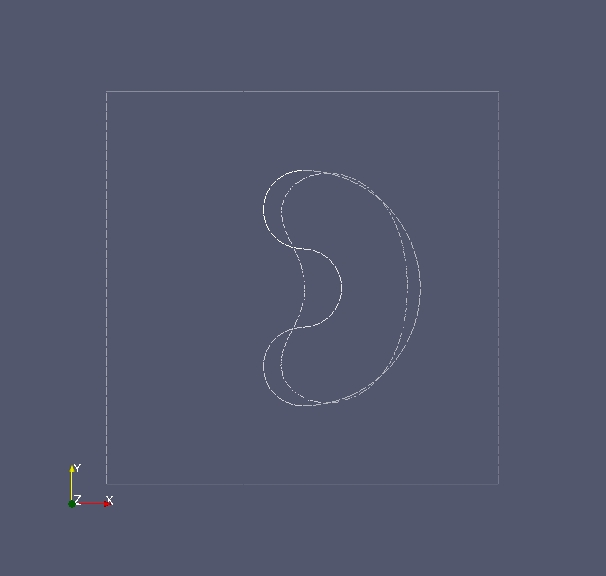
\includegraphics[scale=0.25]{pic_brokendonut_bfgs_linesearch.jpg}
	\caption{}	
	\end{subfigure}
	\begin{subfigure}{0.5\textwidth}
	\centering
	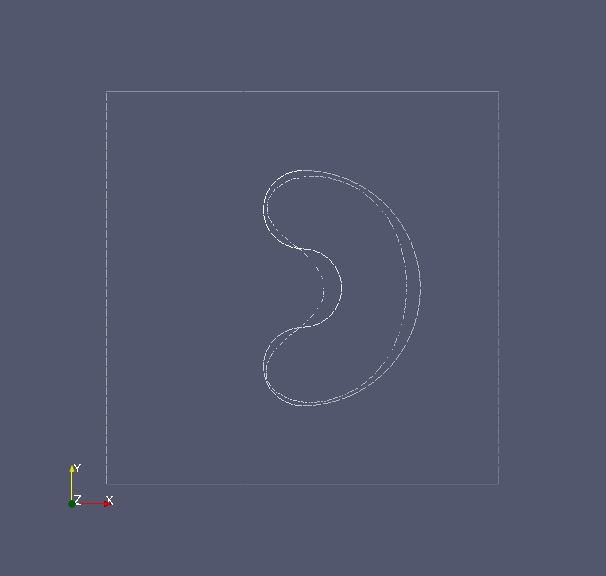
\includegraphics[scale=0.25]{pic_brokendonut_bfgs_linesearch_fine.jpg}
	\caption{}	
	\end{subfigure}
\caption{L-BFGS-Verfahren mit Linesearch (a) Form bei Ausstieg auf grobem Gitter (b) Form bei Ausstieg auf feinem Gitter}
\label{brokendonut_bfgs_linesearch}
\end{figure}


Weiterhin stellen wir fest, dass durch das Weglassen der Perimeter-Regularisierung die Konvergenz in diesem Problem erhalten bleibt, siehe den Graphen \ref{plot_memlen_lame} (b). Lässt man zusätzlich die Lamé-Paramter nicht lokal variieren, so bleibt auch hier die Konvergenz erhalten, das Verfahren benötigt jedoch etwas mehr als die doppelte Anzahl an Schritten bis die Toleranz an die Formableitung unterschritten wird. Betrachtet man die Konvergenzgraphen, fällt jedoch auf, dass dies an dem Ausstiegskriterium liegt, welches etwas zu stark gewählt ist. Somit funktioniert das Verfahren auch unter Anwendung konstanter Lamé-Parameter, sowie bei komplettem Weglassen der Perimeter-Regularisierung, erneut zu sehen in Abbildung \ref{plot_memlen_lame} (b). Allerdings liegt in allen Fällen ohne Linesearch Divergenz vor. Werden lediglich die Lamé-Parameter konstant gehalten, so tritt keine Änderung des Konvergenzverhaltens auf, was auch in Abbildung \ref{plot_memlen_lame} (b) zu sehen ist. Allerdings weisen die Zellen ohne lokal-variierende Lamé-Parameter einen höheren Entartungsgrad auf.

Außerdem beobachten wir, dass bei einer Memory-Length von 3, sprich bei einem echten Limited-Memory Ansatz, die Anzahl der benötigten Schritte zur Konvergenz von 26 auf 35 auf dem feinen Gitter steigt, jedoch bei dem groben Gitter gleich bei 8 Schritten bleibt. 

Zuletzt möchten wir anmerken, dass bei Betrachtung aller Konvergenzgraphen des BFGS-Verfahrens, sowohl des ersten Problems \ref{Konvplots_circle}, als auch des zweiten Problems \ref{plot_konvergenzdonut}, eine erhebliche, sprungartige Verbesserung im zweiten Schritt erfolgt. Wir vermuten, dass dies durch die Verwandtschaft des L-BFGS-Verfahrens mit dem CG-Verfahren erklärbar ist. Die Autoren von \cite{bfgsjumpconv} zeigen für die Minimierung quadratischer Zielfunktionen im $\mathbb{R}^n$ unter gewissen Bedingungen, dass alle Mitglieder der Broyden-Klasse, somit auch das BFGS-Verfahren, bei vollen Updates nach nur $n$ Schritten die Lösung erreichen. Verwenden die Autoren die Limited-Memory-Varianten, so verlieren alle Mitglieder der Broyden-Klasse diese Eigenschaft, mit einziger Ausnahme des L-BFGS-Verfahrens. Weiterhin zeigen die Autoren, dass bei der auch von uns angewandten Skipping-Strategie, dem Aussetzen von Updates bei Verletzung der Curvature-Condition, bei $q$-maligem Aussetzen immer noch ein Erreichen der Lösung nach nur $n+q$ Schritten vorliegt. Zwar haben die Autoren dies wie erwähnt für quadratische Funktionen im $\mathbb{R}^n$ gezeigt, unsere Beobachtungen bei den genannten Konvergenzgraphen legen jedoch ein ähnliches Verhalten in Kontext der Formoptimierung nahe. 

Wir beenden nun die Analyse der von uns erzeugten Daten, und laden die Leser dieser Arbeit gerne dazu ein, dass beiliegende Programm bei Interesse selber einigen Tests zu unterziehen. Abschließend möchten wir einen kleinen Ausblick auf mögliche weiterführende Themen und einige Probleme geben.

\subsection{Ausblick und Schlussbetrachtung}
Wir haben mit der in Kapitel \ref{Chapter_implementation} vorgestellten Implementierung, und den Ergebnissen aus den Abschnitten \ref{subsect_circle} und \ref{subsect_donut}, ein durchaus effektives Quasi-Newton-Verfahren in der Formoptimierung demonstriert. 
Die Konvergenzgeschwindigkeit im Vergleich zum Gradientenverfahren ist deutlich erhöht. Wir haben gesehen, dass eine Art der Schrittweitensteuerung, etwa dem bei uns implementierten Backtracking-Linesearch, für die Konvergenz des L-BFGS-Verfahrens nötig ist. An dieser Stelle gibt es Bedarf für weitere Entwicklungen; so wäre entweder eine im vorigen Kapitel angesprochene Verbesserung des Kriteriums für hinreichend gute Abstiege, die ein aus dem Formkalkül legitimes Modell für das Zielfunktional verwenden, denkbar. Diese könnte im Falle eines linearen Modells das Armijo-Kriterium auf Formräume verallgemeinern. Eine andere Variante wäre die Verwendung einer Art Trust-Region-Methode, mit dessen Hilfe auch eine globale Konvergenz erreicht werden könnte. Zudem kann sich mit diesem Ansatz die Möglichkeit bieten, durch das Vermeiden der Indefinitheit der Quasi-Newton-Approximation andere Verfahren, etwa den Broyden-SR1-Update, anwenden zu können. In den Konvergenzgraphen sind außerdem deutliche Verbesserungen nach nur wenigen Schritten zu erkennen, welche wir zuvor versucht haben zu erklären, und eine Ähnlichkeit zum CG-Verfahren ausweisen. Eine Limited-Memory-Variante des CG-Verfahrens für die Formoptimierung wäre eine weitere Möglichkeit dem zuvor genannten Problemen zu begegnen. Außerdem haben wir keine asymptotisch superlineare Konvergenz beobachten oder zuverlässig widerlegen können. Um dies anzugehen, wäre eine Anpassung der BFGS-Updates wichtig. Wie sich diese konkret im Formraum realisieren lässt, ist jedoch bis dato unklar. Wir haben weiterhin Indizien für gitterunabhängige Konvergenz bei Untersuchung des Gradientenverfahrens bemerkt, so dass es sich lohnenswert erscheint, das Verhalten der Verfahren bei anderen Problemen und anderer Wahl der Bilinearform $a$ und der damit erhaltenen Metrik $g^S$ zu analysieren. Eine Möglichkeit hierfür würde die biharmonische Gleichung bieten. Abschließend bleibt noch das etwas ominöse Problem bei Erzeugung der Formgradienten, bei dem ohne Nullsetzen der Punkte ohne Träger am inneren Rand zur Lösung der linearen Elastizitätsgleichung die verheerenden Effekte auftreten, welche das Gitter zerstören und wir nicht befriedigend erklären können. Dies sind viele mögliche Ansätze für kommende  Fortschritte im Bereich der Formoptimierung. Wir hoffen, mit dieser Arbeit einen kleinen Beitrag in die richtige Richtung gegeben zu haben, und bedanken uns bei Prof. Volker Schulz für die Möglichkeit diese Masterarbeit anzufertigen.
\newpage
\nocite{*}
\bibliographystyle{plain}
\bibliography{papers}

\end{document}
